\begin{figure}[h]
	\centering
	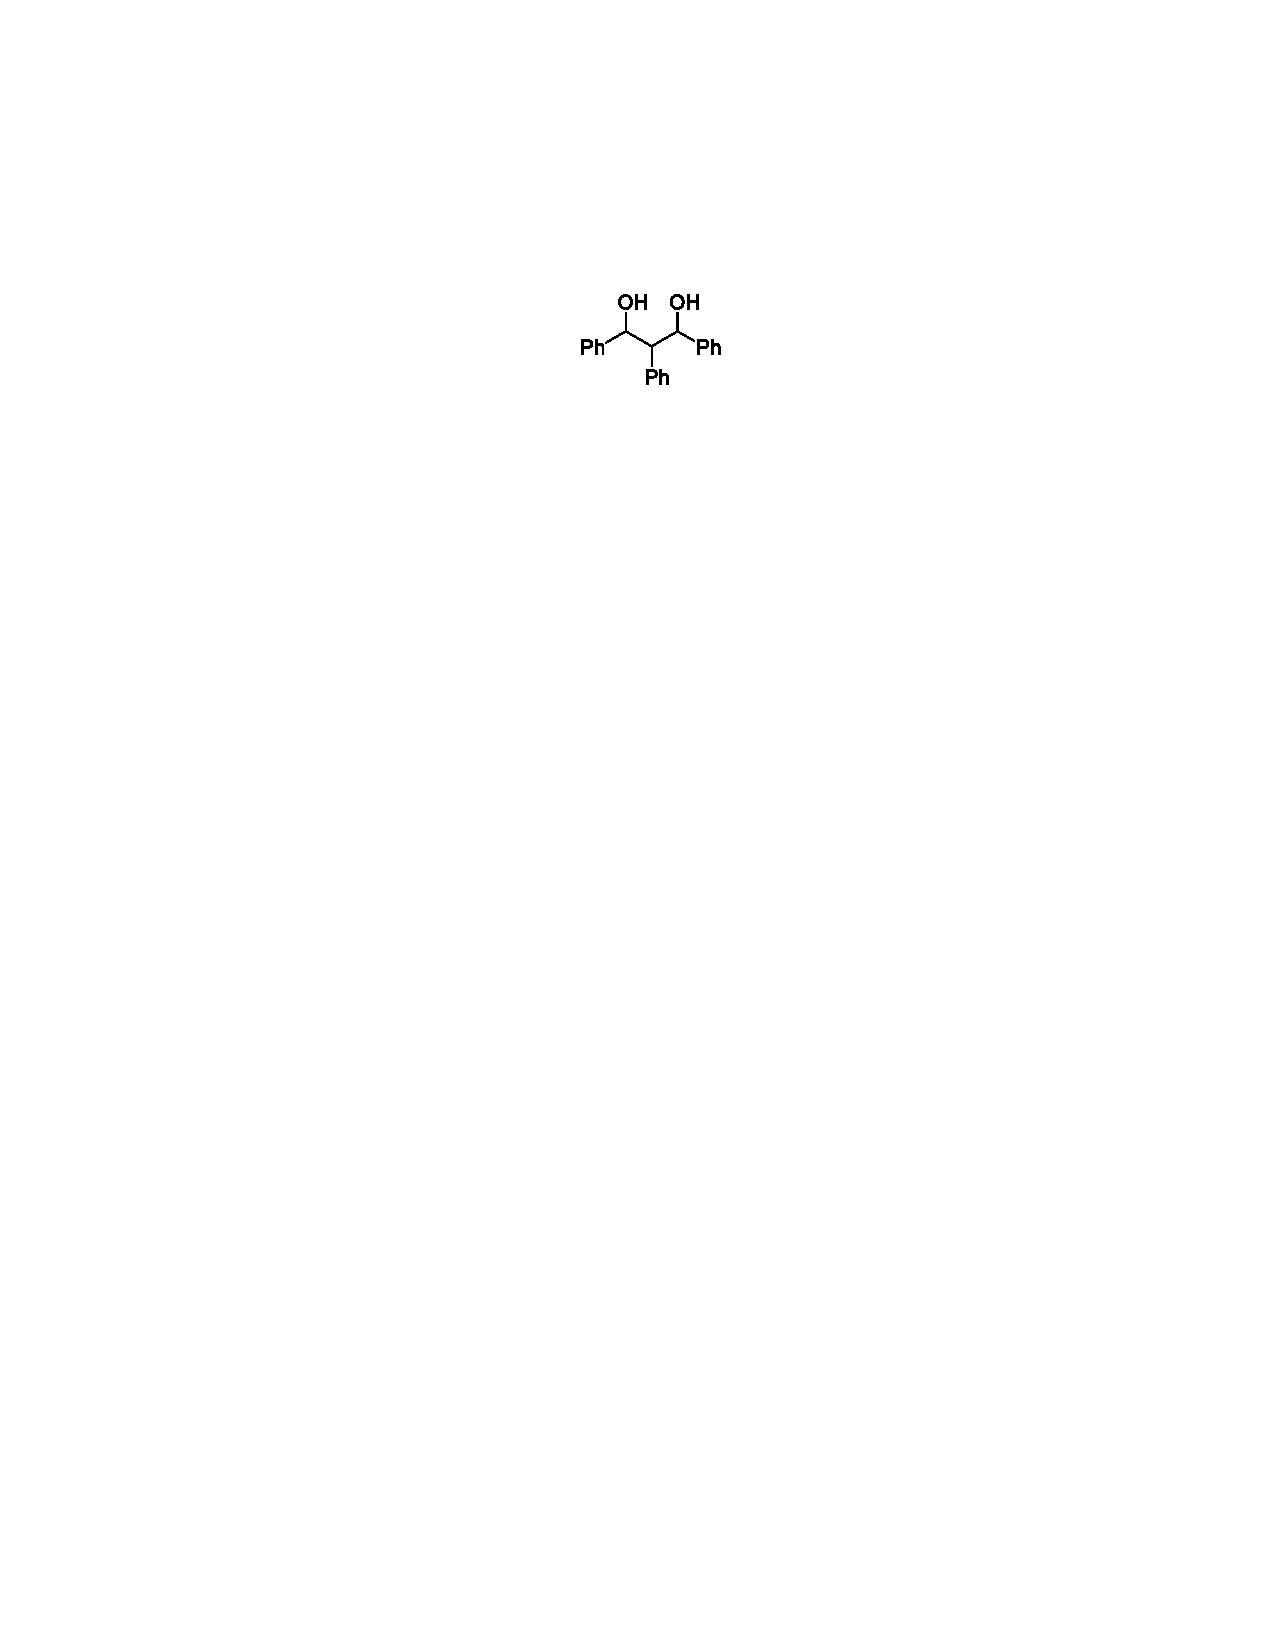
\includegraphics[width=5cm]{./pic/t8-1.pdf}
\end{figure}

\noindent\textbf{8.1.} 画出1,2,3-三苯基丙-1,3-二醇的所有立体异构体。

\noindent\textbf{8.2.} 列出其中所有的非手性化合物。

\noindent\textbf{8.3.} 列出其中所有的手性化合物。

\noindent\textbf{8.4.} 下列哪一些性质或者方法可以用来区分问题8.3中的手性化合物?选择所有正确的观点。

\renewcommand{\labelitemi}{$\square$}
\begin{itemize}
\item 沸点
\item 紫外光谱
\item 折射率
\item 熔点
\item 旋光度
\item 偶极矩
\item 非手性环境中的核磁共振
\item 红外光谱
\end{itemize}
\renewcommand{\labelitemi}{$\bullet$}
